% Options for packages loaded elsewhere
\PassOptionsToPackage{unicode}{hyperref}
\PassOptionsToPackage{hyphens}{url}
%
\documentclass[
]{book}
\usepackage{amsmath,amssymb}
\usepackage{lmodern}
\usepackage{iftex}
\ifPDFTeX
  \usepackage[T1]{fontenc}
  \usepackage[utf8]{inputenc}
  \usepackage{textcomp} % provide euro and other symbols
\else % if luatex or xetex
  \usepackage{unicode-math}
  \defaultfontfeatures{Scale=MatchLowercase}
  \defaultfontfeatures[\rmfamily]{Ligatures=TeX,Scale=1}
\fi
% Use upquote if available, for straight quotes in verbatim environments
\IfFileExists{upquote.sty}{\usepackage{upquote}}{}
\IfFileExists{microtype.sty}{% use microtype if available
  \usepackage[]{microtype}
  \UseMicrotypeSet[protrusion]{basicmath} % disable protrusion for tt fonts
}{}
\makeatletter
\@ifundefined{KOMAClassName}{% if non-KOMA class
  \IfFileExists{parskip.sty}{%
    \usepackage{parskip}
  }{% else
    \setlength{\parindent}{0pt}
    \setlength{\parskip}{6pt plus 2pt minus 1pt}}
}{% if KOMA class
  \KOMAoptions{parskip=half}}
\makeatother
\usepackage{xcolor}
\IfFileExists{xurl.sty}{\usepackage{xurl}}{} % add URL line breaks if available
\IfFileExists{bookmark.sty}{\usepackage{bookmark}}{\usepackage{hyperref}}
\hypersetup{
  pdftitle={A primer in Human Cardiovascular Genetics},
  pdfauthor={dr. Sander W. van der Laan \textbar{} swvanderlaan},
  hidelinks,
  pdfcreator={LaTeX via pandoc}}
\urlstyle{same} % disable monospaced font for URLs
\usepackage{longtable,booktabs,array}
\usepackage{calc} % for calculating minipage widths
% Correct order of tables after \paragraph or \subparagraph
\usepackage{etoolbox}
\makeatletter
\patchcmd\longtable{\par}{\if@noskipsec\mbox{}\fi\par}{}{}
\makeatother
% Allow footnotes in longtable head/foot
\IfFileExists{footnotehyper.sty}{\usepackage{footnotehyper}}{\usepackage{footnote}}
\makesavenoteenv{longtable}
\usepackage{graphicx}
\makeatletter
\def\maxwidth{\ifdim\Gin@nat@width>\linewidth\linewidth\else\Gin@nat@width\fi}
\def\maxheight{\ifdim\Gin@nat@height>\textheight\textheight\else\Gin@nat@height\fi}
\makeatother
% Scale images if necessary, so that they will not overflow the page
% margins by default, and it is still possible to overwrite the defaults
% using explicit options in \includegraphics[width, height, ...]{}
\setkeys{Gin}{width=\maxwidth,height=\maxheight,keepaspectratio}
% Set default figure placement to htbp
\makeatletter
\def\fps@figure{htbp}
\makeatother
\setlength{\emergencystretch}{3em} % prevent overfull lines
\providecommand{\tightlist}{%
  \setlength{\itemsep}{0pt}\setlength{\parskip}{0pt}}
\setcounter{secnumdepth}{5}
\usepackage{booktabs}
\usepackage{amsthm}
\makeatletter
\def\thm@space@setup{%
  \thm@preskip=8pt plus 2pt minus 4pt
  \thm@postskip=\thm@preskip
}
\makeatother
\ifLuaTeX
  \usepackage{selnolig}  % disable illegal ligatures
\fi
\usepackage[]{natbib}
\bibliographystyle{apalike}

\title{A primer in Human Cardiovascular Genetics}
\author{\href{https://swvanderlaan.github.iio}{dr. Sander W. van der Laan} \textbar{} \href{https://www.twitter.com/swvanderlaan}{swvanderlaan}}
\date{Last update: 2022-03-24}

\begin{document}
\maketitle

{
\setcounter{tocdepth}{1}
\tableofcontents
}
\hypertarget{about-this-primer}{%
\chapter{About this primer}\label{about-this-primer}}

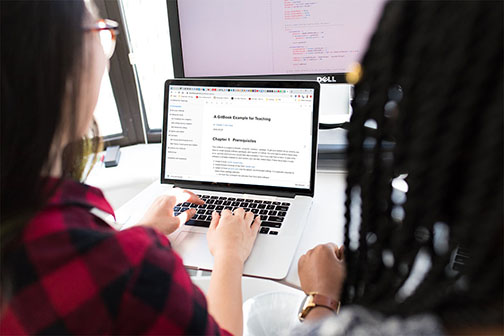
\includegraphics{./img/using_gitbook.jpeg}

\hypertarget{introduction}{%
\section{Introduction}\label{introduction}}

Welcome to the \emph{A primer in Human Cardiovascular Genetics} as part of the \textbf{Genetic Epidemiology} course. In the next few days we will use this \href{https://cjvanlissa.github.io/gitbook-demo/}{GitBook} to perform quality control (QC), executing a genome-wide association study (GWAS), annotating the GWAS results, and performing further downstream analyses. We will use data from the first release of the \href{https://www.wtccc.org.uk/ccc1/overview.html}{\emph{Welcome Trust Case-Control Consortium (WTCCC)}} and focus on coronary artery disease (CAD).

Unfortunately, during this course there is no time to perform \href{https://www.nature.com/articles/nrg2796}{imputation}, but I will provide some pointers during the course as to how to do this with minimal coding/scripting experience. Likewise, this practical does not cover the aspects of meta-analyses of GWAS. But rest assured, I will add chapters on these subjects to a future version.

\hypertarget{background-reading}{%
\section{Background reading}\label{background-reading}}

Part of this is based on four great Nature Protocols from the \href{https://www.well.ox.ac.uk/research/research-groups/zondervan-group}{Zondervan group} at the Wellcome Center Human Genetics.

\begin{enumerate}
\def\labelenumi{\arabic{enumi}.}
\tightlist
\item
  \href{https://www.ncbi.nlm.nih.gov/pubmed/17947991}{Zondervan KT \emph{et al.} \emph{Designing candidate gene and genome-wide case-control association studies.} Nat Protoc 2007.}
\item
  \href{https://www.ncbi.nlm.nih.gov/pubmed/19390530}{Pettersson FH \emph{et al.} \emph{Marker selection for genetic case-control association studies.} Nat Protoc 2009.}
\item
  \href{https://www.ncbi.nlm.nih.gov/pubmed/21085122}{Anderson CA \emph{et al.} \emph{Data QC in genetic case-control association studies.} Nat Protoc 2010.}
\item
  \href{https://www.ncbi.nlm.nih.gov/pubmed/21293453}{Clarke GM \emph{et al.} \emph{Basic statistical analysis in genetic case-control studies.} Nat Protoc 2011.}
\end{enumerate}

An update on the community standards of QC for GWAS can be found here:

\begin{enumerate}
\def\labelenumi{\arabic{enumi}.}
\tightlist
\item
  \href{https://www.ncbi.nlm.nih.gov/pubmed/20718045}{Laurie CC \emph{et al.} \emph{Quality control and quality assurance in genotypic data for genome-wide association studies.} Genet Epidemiol 2010.}
\end{enumerate}

With respect to imputation you should also get familiar with the following two works:

\begin{enumerate}
\def\labelenumi{\arabic{enumi}.}
\tightlist
\item
  \href{https://doi.org/10.1038/nrg2796}{Marchini, J. and Howie, B. \emph{Genotype imputation for genome-wide association studies.} Nat Rev Genet 2010}
\item
  \href{https://www.ncbi.nlm.nih.gov/pubmed/18852200}{de Bakker PIW \emph{et al.} \emph{Practical aspects of imputation-driven meta-analysis of genome-wide association studies.} Hum Mol Genet 2008.}
\item
  \href{https://www.ncbi.nlm.nih.gov/pubmed/24762786}{Winkler TW \emph{et al.} \emph{Quality control and conduct of genome-wide association meta-analyses.} Nat Protoc 2014.}
\end{enumerate}

\hypertarget{meet-the-team}{%
\section{Meet the Team}\label{meet-the-team}}

We work with a team of enthusiastic lecturers with experience in bioinformatics, GWAS, genetic analyses, Mendelian randomization, and epidemiology. This year the team consists of:

\begin{longtable}[]{@{}
  >{\raggedright\arraybackslash}p{(\columnwidth - 0\tabcolsep) * \real{0.2083}}@{}}
\toprule
\endhead
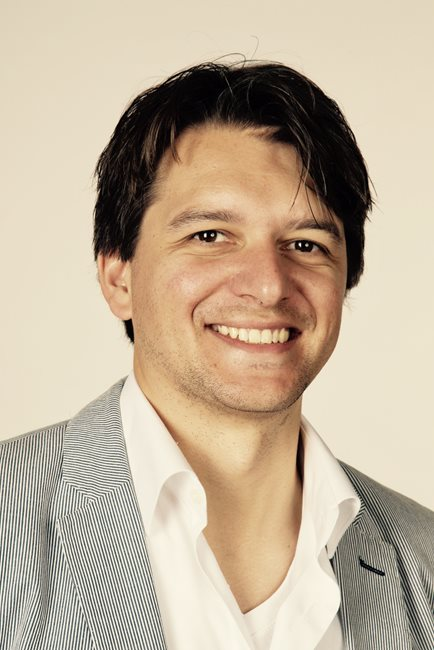
\includegraphics[width=0.15\textwidth,height=\textheight]{img/_team/sander_vander_laan.jpg} Sander W. van der Laan \emph{Assistant professor}Course coordinator\href{mailto:s.w.vanderlaan-2@umcutrecht.nl}{\nolinkurl{s.w.vanderlaan-2@umcutrecht.nl}} \textbar{} \href{http://www.twitter.com/swvanderlaan}{swvanderlaan} \\
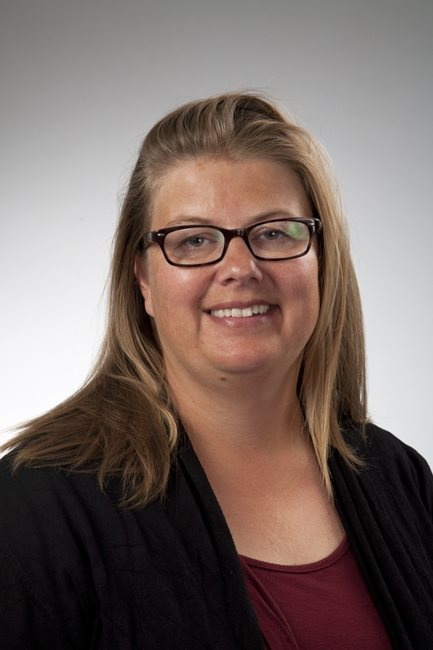
\includegraphics[width=0.15\textwidth,height=\textheight]{img/_team/charlotte_onland.jpg} Charlotte Onland-Moret \emph{Associate Professor}\href{mailto:N.C.Onland@umcutrecht.nl}{\nolinkurl{N.C.Onland@umcutrecht.nl}} \\
\href{img/_team/jessica_van_setten.jpg}{} Jessica van Setten \emph{Assistant professor}\href{mailto:j.vansetten@umcutrecht.nl}{\nolinkurl{j.vansetten@umcutrecht.nl}} \textbar{} \href{http://www.twitter.com/j_vansetten}{j\_vansetten} \\
 \\
 \\
\bottomrule
\end{longtable}

\hypertarget{final-thoughts}{%
\section{Final thoughts}\label{final-thoughts}}

I can imagine this seems overwhelming, but trust me, you'll be okay. Just follow this practical, but also work on the questions asked during the lectures and in this practical. You'll learn by doing and at the end of the day, you can execute a GWAS independently.

Ready to start?

Your first point of action is to prepare your system for this course (Chapter \ref{prerequisites}).

\hypertarget{prerequisites}{%
\chapter{Prerequisites}\label{prerequisites}}

\hypertarget{linux-macos-and-windows}{%
\section{Linux, macOS, and Windows}\label{linux-macos-and-windows}}

Most programs made to execute genetic studies are developed for the Unix environment, \emph{e.g.} Linux and macOS. Therefore, they may not work as intended on window's environment. Fortunately, Windows now allow users to install a linux subsystem within Windows 10 and you can find the detail \href{https://docs.microsoft.com/en-us/windows/wsl/about}{guide} here.\\
However, we highly recommend to 1) either install a linux subsystem on your Windows computer (\emph{e.g.} \href{https://blog.storagecraft.com/the-dead-simple-guide-to-installing-a-linux-virtual-machine-on-windows/}{a virtual machine with Ubuntu could work}), or 2) switch to macOS in combination with \href{https://brew.sh}{homebrew} as this will give you advantage of a powerful computer with a userfriendly interface and all the flexibility to use Unix-based programs for your work.

\begin{quote}
For this practical we use a Windows laptop with Ubuntu on a VirtualMachine. Therefore every command is intended for Linux/macOS.
\end{quote}

\hypertarget{programs-you-need}{%
\section{Programs you need}\label{programs-you-need}}

You need few programs for this practical or for your (future) genetic epidemiology work for that matter.

\begin{longtable}[]{@{}
  >{\raggedright\arraybackslash}p{(\columnwidth - 4\tabcolsep) * \real{0.1667}}
  >{\raggedright\arraybackslash}p{(\columnwidth - 4\tabcolsep) * \real{0.1111}}
  >{\raggedright\arraybackslash}p{(\columnwidth - 4\tabcolsep) * \real{0.5694}}@{}}
\toprule
\begin{minipage}[b]{\linewidth}\raggedright
Program
\end{minipage} & \begin{minipage}[b]{\linewidth}\raggedright
Link
\end{minipage} & \begin{minipage}[b]{\linewidth}\raggedright
Description
\end{minipage} \\
\midrule
\endhead
PLINK & {[}\url{https:/} & /www.cog-genomics.org/plink2/{]}(\url{https://www.cog-genomics.org/plink2/})\{target=``\_blank''\} PLINK is a free, open-source genetic analysis toolset, designed to perform a range of basic data parsing and quality control, as well as basic and large-scale analyses in a computationally efficient manner. \\
R & {[}\url{https:/} & /cran.r-project.org{]}(\url{https://cran.r-project.org/})\{target=``\_blank''\} Progam to perform statistical analysis and visualisations. \\
RStudio & {[}\url{https:/} & /www.rstudio.com{]}(\url{https://www.rstudio.com})\{target=``\_blank''\} A userfriendly R-wrap-around for code editing, debugging, analyses, and visualisation \\
\bottomrule
\end{longtable}

Table 1: Programs needed for genetic epidemiology.

All genetic analyses can be done in PLINK, even on your laptop, but with large datasets, e.g.~UK-biobank size, it's better to switch to a \href{https://wiki.bioinformatics.umcutrecht.nl/bin/view/HPC/WebHome}{high-performance computing cluster} like we have at the Uithof.

Nowadays, a lot of people also use programs like \href{snptest}{SNPTEST}, \href{https://data.broadinstitute.org/alkesgroup/BOLT-LMM/}{BOLT-LMM}, and \href{http://cnsgenomics.com/software/gcta/\#Overview}{GCTA} as alternatives to run GWAS and downstream analyses, \emph{e.g.} heritability estimation, Fst-calculation, etc.

Mendelian randomisation can be done either with the \href{http://cnsgenomics.com/software/smr/\#Overview}{SMR} or \href{http://cnsgenomics.com/software/gsmr/}{GSMR} function from GCTA or with R-packages, like \texttt{TwoSampleMR}.

\hypertarget{the-terminal}{%
\section{The Terminal}\label{the-terminal}}

For all the above programs, except RStudio, you will need the \texttt{Terminal}. This comes with every major operating system. And you will (start to) make your own scripts. The benefit of using scripts is that each step is clearly layed out and easily replicable, thus allows for greater reproducibility, easier troubleshooting and can be run on high-performance computer clusters.

Download the data you need to your Desktop: LINK.

Now open the terminal, it should be on the left in the toolbar as a little black computer-monitor-like icon.
Mac uses can type \texttt{command\ +\ space} and type \texttt{terminal}, a terminal screen should open.

\begin{quote}
From now on we will use little code blocks like the example to indicate a code you should type/copy-paste and hit enter. If a code is followed by a comment, it is indicated by a \# - you don't need to copy-paste and execute this.
\end{quote}

\begin{verbatim}
CODE BLOCK

CODE BLOCK # some comment here

\end{verbatim}

You can navigate around the computer through the terminal by typing \texttt{cd\ \textless{}path\textgreater{}}; \texttt{cd} stands for ``change directory'' and means ``some\_file\_directory\_you\_want\_to\_go\_to''.

\begin{verbatim}
# For Linux/macOS Users
cd ~ # will bring you to your home directory
cd ../ # will bring you to the parent directory (up one level) 
cd XXX # will bring you to the XXX directory
\end{verbatim}

Let's navigate to the folder you just downloaded.

\begin{verbatim}
cd ~/Desktop/practical
\end{verbatim}

Let's check out what is inside the directory, by listing (\texttt{ls}) its contents.

\begin{verbatim}
ls -lh

# For Linux/macOS Users
ls -l # shows files as list
ls -lh # shows files as list with human readable format 
ls -lt # shows the files as list sorted by time edited
ls -lS # shows the files as list sorted by size
\end{verbatim}

Adding the flags \texttt{-lh} will get you the contents of a directory in a list (\texttt{-l}) and make the size `human-readable' (\texttt{-h}).

You can also count the number of files.

\begin{verbatim}
ls | wc -l
\end{verbatim}

\hypertarget{installing-some-r-packages}{%
\section{Installing some R packages}\label{installing-some-r-packages}}

I tested this VirtualMachine and everything should be fine, except some libraries weren't there. We need to install them.

To be able to install certain \texttt{r}-packages, we need to install some Linux (Ubuntu) software. Type the following:

\begin{verbatim}
sudo apt-get install libcurl4 libcurl4-openssl-dev -y

sudo apt-get install libssl-dev
\end{verbatim}

Now close the terminal window - really making sure that the terminal-program has quit.

Open a new terminal window and open \texttt{r} by simply typing \texttt{R}. You should install the following packages, and then you're good to go!

\begin{verbatim}
install.packages(c("httr", "usethis", "data.table", "devtools", "qqman", "CMplot", "tibble", "plotly", "dplyr"))

library(c("httr", "usethis", "data.table", "devtools", "qqman", "CMplot", "tibble", "plotly", "dplyr"))
devtools::install_github("kassambara/ggpubr")
library("ggpubr")
\end{verbatim}

All in all this may take some time, good moment to relax, review your notes, stretch your legs, or take a coffee.

\hypertarget{basics-of-a-genome-wide-association-study-gwas}{%
\chapter{Basics of a Genome-Wide Association Study (GWAS)}\label{basics-of-a-genome-wide-association-study-gwas}}

\hypertarget{section-1}{%
\section{Section 1}\label{section-1}}

Lorem ipsum dolor sit amet, consectetur adipiscing elit, sed do eiusmod tempor incididunt ut labore et dolore magna aliqua. Ut enim ad minim veniam, quis nostrud exercitation ullamco laboris nisi ut aliquip ex ea commodo consequat. Duis aute irure dolor in reprehenderit in voluptate velit esse cillum dolore eu fugiat nulla pariatur. Excepteur sint occaecat cupidatat non proident, sunt in culpa qui officia deserunt mollit anim id est laborum.

\hypertarget{section-2}{%
\section{Section 2}\label{section-2}}

Sed ut perspiciatis unde omnis iste natus error sit voluptatem accusantium doloremque laudantium, totam rem aperiam, eaque ipsa quae ab illo inventore veritatis et quasi architecto beatae vitae dicta sunt explicabo. Nemo enim ipsam voluptatem quia voluptas sit aspernatur aut odit aut fugit, sed quia consequuntur magni dolores eos qui ratione voluptatem sequi nesciunt. Neque porro quisquam est, qui dolorem ipsum quia dolor sit amet, consectetur, adipisci velit, sed quia non numquam eius modi tempora incidunt ut labore et dolore magnam aliquam quaerat voluptatem. Ut enim ad minima veniam, quis nostrum exercitationem ullam corporis suscipit laboriosam, nisi ut aliquid ex ea commodi consequatur? Quis autem vel eum iure reprehenderit qui in ea voluptate velit esse quam nihil molestiae consequatur, vel illum qui dolorem eum fugiat quo voluptas nulla pariatur?

\hypertarget{section-3}{%
\section{Section 3}\label{section-3}}

At vero eos et accusamus et iusto odio dignissimos ducimus qui blanditiis praesentium voluptatum deleniti atque corrupti quos dolores et quas molestias excepturi sint occaecati cupiditate non provident, similique sunt in culpa qui officia deserunt mollitia animi, id est laborum et dolorum fuga. Et harum quidem rerum facilis est et expedita distinctio. Nam libero tempore, cum soluta nobis est eligendi optio cumque nihil impedit quo minus id quod maxime placeat facere possimus, omnis voluptas assumenda est, omnis dolor repellendus. Temporibus autem quibusdam et aut officiis debitis aut rerum necessitatibus saepe eveniet ut et voluptates repudiandae sint et molestiae non recusandae. Itaque earum rerum hic tenetur a sapiente delectus, ut aut reiciendis voluptatibus maiores alias consequatur aut perferendis doloribus asperiores repellat.

\hypertarget{wtccc1-a-gwas-on-coronary-artery-disease-cad}{%
\chapter{WTCCC1: a GWAS on coronary artery disease (CAD)}\label{wtccc1-a-gwas-on-coronary-artery-disease-cad}}

\hypertarget{section-1-1}{%
\section{Section 1}\label{section-1-1}}

Lorem ipsum dolor sit amet, consectetur adipiscing elit, sed do eiusmod tempor incididunt ut labore et dolore magna aliqua. Ut enim ad minim veniam, quis nostrud exercitation ullamco laboris nisi ut aliquip ex ea commodo consequat. Duis aute irure dolor in reprehenderit in voluptate velit esse cillum dolore eu fugiat nulla pariatur. Excepteur sint occaecat cupidatat non proident, sunt in culpa qui officia deserunt mollit anim id est laborum.

\hypertarget{section-2-1}{%
\section{Section 2}\label{section-2-1}}

Sed ut perspiciatis unde omnis iste natus error sit voluptatem accusantium doloremque laudantium, totam rem aperiam, eaque ipsa quae ab illo inventore veritatis et quasi architecto beatae vitae dicta sunt explicabo. Nemo enim ipsam voluptatem quia voluptas sit aspernatur aut odit aut fugit, sed quia consequuntur magni dolores eos qui ratione voluptatem sequi nesciunt. Neque porro quisquam est, qui dolorem ipsum quia dolor sit amet, consectetur, adipisci velit, sed quia non numquam eius modi tempora incidunt ut labore et dolore magnam aliquam quaerat voluptatem. Ut enim ad minima veniam, quis nostrum exercitationem ullam corporis suscipit laboriosam, nisi ut aliquid ex ea commodi consequatur? Quis autem vel eum iure reprehenderit qui in ea voluptate velit esse quam nihil molestiae consequatur, vel illum qui dolorem eum fugiat quo voluptas nulla pariatur?

\hypertarget{section-3-1}{%
\section{Section 3}\label{section-3-1}}

At vero eos et accusamus et iusto odio dignissimos ducimus qui blanditiis praesentium voluptatum deleniti atque corrupti quos dolores et quas molestias excepturi sint occaecati cupiditate non provident, similique sunt in culpa qui officia deserunt mollitia animi, id est laborum et dolorum fuga. Et harum quidem rerum facilis est et expedita distinctio. Nam libero tempore, cum soluta nobis est eligendi optio cumque nihil impedit quo minus id quod maxime placeat facere possimus, omnis voluptas assumenda est, omnis dolor repellendus. Temporibus autem quibusdam et aut officiis debitis aut rerum necessitatibus saepe eveniet ut et voluptates repudiandae sint et molestiae non recusandae. Itaque earum rerum hic tenetur a sapiente delectus, ut aut reiciendis voluptatibus maiores alias consequatur aut perferendis doloribus asperiores repellat.

\hypertarget{post-gwas-analyses}{%
\chapter{Post-GWAS Analyses}\label{post-gwas-analyses}}

\hypertarget{section-1-2}{%
\section{Section 1}\label{section-1-2}}

Lorem ipsum dolor sit amet, consectetur adipiscing elit, sed do eiusmod tempor incididunt ut labore et dolore magna aliqua. Ut enim ad minim veniam, quis nostrud exercitation ullamco laboris nisi ut aliquip ex ea commodo consequat. Duis aute irure dolor in reprehenderit in voluptate velit esse cillum dolore eu fugiat nulla pariatur. Excepteur sint occaecat cupidatat non proident, sunt in culpa qui officia deserunt mollit anim id est laborum.

\hypertarget{section-2-2}{%
\section{Section 2}\label{section-2-2}}

Sed ut perspiciatis unde omnis iste natus error sit voluptatem accusantium doloremque laudantium, totam rem aperiam, eaque ipsa quae ab illo inventore veritatis et quasi architecto beatae vitae dicta sunt explicabo. Nemo enim ipsam voluptatem quia voluptas sit aspernatur aut odit aut fugit, sed quia consequuntur magni dolores eos qui ratione voluptatem sequi nesciunt. Neque porro quisquam est, qui dolorem ipsum quia dolor sit amet, consectetur, adipisci velit, sed quia non numquam eius modi tempora incidunt ut labore et dolore magnam aliquam quaerat voluptatem. Ut enim ad minima veniam, quis nostrum exercitationem ullam corporis suscipit laboriosam, nisi ut aliquid ex ea commodi consequatur? Quis autem vel eum iure reprehenderit qui in ea voluptate velit esse quam nihil molestiae consequatur, vel illum qui dolorem eum fugiat quo voluptas nulla pariatur?

\hypertarget{section-3-2}{%
\section{Section 3}\label{section-3-2}}

At vero eos et accusamus et iusto odio dignissimos ducimus qui blanditiis praesentium voluptatum deleniti atque corrupti quos dolores et quas molestias excepturi sint occaecati cupiditate non provident, similique sunt in culpa qui officia deserunt mollitia animi, id est laborum et dolorum fuga. Et harum quidem rerum facilis est et expedita distinctio. Nam libero tempore, cum soluta nobis est eligendi optio cumque nihil impedit quo minus id quod maxime placeat facere possimus, omnis voluptas assumenda est, omnis dolor repellendus. Temporibus autem quibusdam et aut officiis debitis aut rerum necessitatibus saepe eveniet ut et voluptates repudiandae sint et molestiae non recusandae. Itaque earum rerum hic tenetur a sapiente delectus, ut aut reiciendis voluptatibus maiores alias consequatur aut perferendis doloribus asperiores repellat.

\hypertarget{conditional-analysis}{%
\chapter{Conditional analysis}\label{conditional-analysis}}

\hypertarget{section-1-3}{%
\section{Section 1}\label{section-1-3}}

Lorem ipsum dolor sit amet, consectetur adipiscing elit, sed do eiusmod tempor incididunt ut labore et dolore magna aliqua. Ut enim ad minim veniam, quis nostrud exercitation ullamco laboris nisi ut aliquip ex ea commodo consequat. Duis aute irure dolor in reprehenderit in voluptate velit esse cillum dolore eu fugiat nulla pariatur. Excepteur sint occaecat cupidatat non proident, sunt in culpa qui officia deserunt mollit anim id est laborum.

\hypertarget{section-2-3}{%
\section{Section 2}\label{section-2-3}}

Sed ut perspiciatis unde omnis iste natus error sit voluptatem accusantium doloremque laudantium, totam rem aperiam, eaque ipsa quae ab illo inventore veritatis et quasi architecto beatae vitae dicta sunt explicabo. Nemo enim ipsam voluptatem quia voluptas sit aspernatur aut odit aut fugit, sed quia consequuntur magni dolores eos qui ratione voluptatem sequi nesciunt. Neque porro quisquam est, qui dolorem ipsum quia dolor sit amet, consectetur, adipisci velit, sed quia non numquam eius modi tempora incidunt ut labore et dolore magnam aliquam quaerat voluptatem. Ut enim ad minima veniam, quis nostrum exercitationem ullam corporis suscipit laboriosam, nisi ut aliquid ex ea commodi consequatur? Quis autem vel eum iure reprehenderit qui in ea voluptate velit esse quam nihil molestiae consequatur, vel illum qui dolorem eum fugiat quo voluptas nulla pariatur?

\hypertarget{section-3-3}{%
\section{Section 3}\label{section-3-3}}

At vero eos et accusamus et iusto odio dignissimos ducimus qui blanditiis praesentium voluptatum deleniti atque corrupti quos dolores et quas molestias excepturi sint occaecati cupiditate non provident, similique sunt in culpa qui officia deserunt mollitia animi, id est laborum et dolorum fuga. Et harum quidem rerum facilis est et expedita distinctio. Nam libero tempore, cum soluta nobis est eligendi optio cumque nihil impedit quo minus id quod maxime placeat facere possimus, omnis voluptas assumenda est, omnis dolor repellendus. Temporibus autem quibusdam et aut officiis debitis aut rerum necessitatibus saepe eveniet ut et voluptates repudiandae sint et molestiae non recusandae. Itaque earum rerum hic tenetur a sapiente delectus, ut aut reiciendis voluptatibus maiores alias consequatur aut perferendis doloribus asperiores repellat.

\hypertarget{statistical-finemapping}{%
\chapter{Statistical finemapping}\label{statistical-finemapping}}

\hypertarget{section-1-4}{%
\section{Section 1}\label{section-1-4}}

Lorem ipsum dolor sit amet, consectetur adipiscing elit, sed do eiusmod tempor incididunt ut labore et dolore magna aliqua. Ut enim ad minim veniam, quis nostrud exercitation ullamco laboris nisi ut aliquip ex ea commodo consequat. Duis aute irure dolor in reprehenderit in voluptate velit esse cillum dolore eu fugiat nulla pariatur. Excepteur sint occaecat cupidatat non proident, sunt in culpa qui officia deserunt mollit anim id est laborum.

\hypertarget{section-2-4}{%
\section{Section 2}\label{section-2-4}}

Sed ut perspiciatis unde omnis iste natus error sit voluptatem accusantium doloremque laudantium, totam rem aperiam, eaque ipsa quae ab illo inventore veritatis et quasi architecto beatae vitae dicta sunt explicabo. Nemo enim ipsam voluptatem quia voluptas sit aspernatur aut odit aut fugit, sed quia consequuntur magni dolores eos qui ratione voluptatem sequi nesciunt. Neque porro quisquam est, qui dolorem ipsum quia dolor sit amet, consectetur, adipisci velit, sed quia non numquam eius modi tempora incidunt ut labore et dolore magnam aliquam quaerat voluptatem. Ut enim ad minima veniam, quis nostrum exercitationem ullam corporis suscipit laboriosam, nisi ut aliquid ex ea commodi consequatur? Quis autem vel eum iure reprehenderit qui in ea voluptate velit esse quam nihil molestiae consequatur, vel illum qui dolorem eum fugiat quo voluptas nulla pariatur?

\hypertarget{section-3-4}{%
\section{Section 3}\label{section-3-4}}

At vero eos et accusamus et iusto odio dignissimos ducimus qui blanditiis praesentium voluptatum deleniti atque corrupti quos dolores et quas molestias excepturi sint occaecati cupiditate non provident, similique sunt in culpa qui officia deserunt mollitia animi, id est laborum et dolorum fuga. Et harum quidem rerum facilis est et expedita distinctio. Nam libero tempore, cum soluta nobis est eligendi optio cumque nihil impedit quo minus id quod maxime placeat facere possimus, omnis voluptas assumenda est, omnis dolor repellendus. Temporibus autem quibusdam et aut officiis debitis aut rerum necessitatibus saepe eveniet ut et voluptates repudiandae sint et molestiae non recusandae. Itaque earum rerum hic tenetur a sapiente delectus, ut aut reiciendis voluptatibus maiores alias consequatur aut perferendis doloribus asperiores repellat.

\hypertarget{functional-mapping-and-annotation-of-gwas}{%
\chapter{Functional Mapping and Annotation of GWAS}\label{functional-mapping-and-annotation-of-gwas}}

\hypertarget{section-1-5}{%
\section{Section 1}\label{section-1-5}}

Lorem ipsum dolor sit amet, consectetur adipiscing elit, sed do eiusmod tempor incididunt ut labore et dolore magna aliqua. Ut enim ad minim veniam, quis nostrud exercitation ullamco laboris nisi ut aliquip ex ea commodo consequat. Duis aute irure dolor in reprehenderit in voluptate velit esse cillum dolore eu fugiat nulla pariatur. Excepteur sint occaecat cupidatat non proident, sunt in culpa qui officia deserunt mollit anim id est laborum.

\hypertarget{section-2-5}{%
\section{Section 2}\label{section-2-5}}

Sed ut perspiciatis unde omnis iste natus error sit voluptatem accusantium doloremque laudantium, totam rem aperiam, eaque ipsa quae ab illo inventore veritatis et quasi architecto beatae vitae dicta sunt explicabo. Nemo enim ipsam voluptatem quia voluptas sit aspernatur aut odit aut fugit, sed quia consequuntur magni dolores eos qui ratione voluptatem sequi nesciunt. Neque porro quisquam est, qui dolorem ipsum quia dolor sit amet, consectetur, adipisci velit, sed quia non numquam eius modi tempora incidunt ut labore et dolore magnam aliquam quaerat voluptatem. Ut enim ad minima veniam, quis nostrum exercitationem ullam corporis suscipit laboriosam, nisi ut aliquid ex ea commodi consequatur? Quis autem vel eum iure reprehenderit qui in ea voluptate velit esse quam nihil molestiae consequatur, vel illum qui dolorem eum fugiat quo voluptas nulla pariatur?

\hypertarget{section-3-5}{%
\section{Section 3}\label{section-3-5}}

At vero eos et accusamus et iusto odio dignissimos ducimus qui blanditiis praesentium voluptatum deleniti atque corrupti quos dolores et quas molestias excepturi sint occaecati cupiditate non provident, similique sunt in culpa qui officia deserunt mollitia animi, id est laborum et dolorum fuga. Et harum quidem rerum facilis est et expedita distinctio. Nam libero tempore, cum soluta nobis est eligendi optio cumque nihil impedit quo minus id quod maxime placeat facere possimus, omnis voluptas assumenda est, omnis dolor repellendus. Temporibus autem quibusdam et aut officiis debitis aut rerum necessitatibus saepe eveniet ut et voluptates repudiandae sint et molestiae non recusandae. Itaque earum rerum hic tenetur a sapiente delectus, ut aut reiciendis voluptatibus maiores alias consequatur aut perferendis doloribus asperiores repellat.

\hypertarget{phenome-wide-association-study-phewas}{%
\chapter{Phenome-Wide Association Study (PheWAS)}\label{phenome-wide-association-study-phewas}}

\hypertarget{section-1-6}{%
\section{Section 1}\label{section-1-6}}

Lorem ipsum dolor sit amet, consectetur adipiscing elit, sed do eiusmod tempor incididunt ut labore et dolore magna aliqua. Ut enim ad minim veniam, quis nostrud exercitation ullamco laboris nisi ut aliquip ex ea commodo consequat. Duis aute irure dolor in reprehenderit in voluptate velit esse cillum dolore eu fugiat nulla pariatur. Excepteur sint occaecat cupidatat non proident, sunt in culpa qui officia deserunt mollit anim id est laborum.

\hypertarget{section-2-6}{%
\section{Section 2}\label{section-2-6}}

Sed ut perspiciatis unde omnis iste natus error sit voluptatem accusantium doloremque laudantium, totam rem aperiam, eaque ipsa quae ab illo inventore veritatis et quasi architecto beatae vitae dicta sunt explicabo. Nemo enim ipsam voluptatem quia voluptas sit aspernatur aut odit aut fugit, sed quia consequuntur magni dolores eos qui ratione voluptatem sequi nesciunt. Neque porro quisquam est, qui dolorem ipsum quia dolor sit amet, consectetur, adipisci velit, sed quia non numquam eius modi tempora incidunt ut labore et dolore magnam aliquam quaerat voluptatem. Ut enim ad minima veniam, quis nostrum exercitationem ullam corporis suscipit laboriosam, nisi ut aliquid ex ea commodi consequatur? Quis autem vel eum iure reprehenderit qui in ea voluptate velit esse quam nihil molestiae consequatur, vel illum qui dolorem eum fugiat quo voluptas nulla pariatur?

\hypertarget{section-3-6}{%
\section{Section 3}\label{section-3-6}}

At vero eos et accusamus et iusto odio dignissimos ducimus qui blanditiis praesentium voluptatum deleniti atque corrupti quos dolores et quas molestias excepturi sint occaecati cupiditate non provident, similique sunt in culpa qui officia deserunt mollitia animi, id est laborum et dolorum fuga. Et harum quidem rerum facilis est et expedita distinctio. Nam libero tempore, cum soluta nobis est eligendi optio cumque nihil impedit quo minus id quod maxime placeat facere possimus, omnis voluptas assumenda est, omnis dolor repellendus. Temporibus autem quibusdam et aut officiis debitis aut rerum necessitatibus saepe eveniet ut et voluptates repudiandae sint et molestiae non recusandae. Itaque earum rerum hic tenetur a sapiente delectus, ut aut reiciendis voluptatibus maiores alias consequatur aut perferendis doloribus asperiores repellat.

\hypertarget{mendelian-randomization-mr}{%
\chapter{Mendelian Randomization (MR)}\label{mendelian-randomization-mr}}

\hypertarget{section-1-7}{%
\section{Section 1}\label{section-1-7}}

Lorem ipsum dolor sit amet, consectetur adipiscing elit, sed do eiusmod tempor incididunt ut labore et dolore magna aliqua. Ut enim ad minim veniam, quis nostrud exercitation ullamco laboris nisi ut aliquip ex ea commodo consequat. Duis aute irure dolor in reprehenderit in voluptate velit esse cillum dolore eu fugiat nulla pariatur. Excepteur sint occaecat cupidatat non proident, sunt in culpa qui officia deserunt mollit anim id est laborum.

\hypertarget{section-2-7}{%
\section{Section 2}\label{section-2-7}}

Sed ut perspiciatis unde omnis iste natus error sit voluptatem accusantium doloremque laudantium, totam rem aperiam, eaque ipsa quae ab illo inventore veritatis et quasi architecto beatae vitae dicta sunt explicabo. Nemo enim ipsam voluptatem quia voluptas sit aspernatur aut odit aut fugit, sed quia consequuntur magni dolores eos qui ratione voluptatem sequi nesciunt. Neque porro quisquam est, qui dolorem ipsum quia dolor sit amet, consectetur, adipisci velit, sed quia non numquam eius modi tempora incidunt ut labore et dolore magnam aliquam quaerat voluptatem. Ut enim ad minima veniam, quis nostrum exercitationem ullam corporis suscipit laboriosam, nisi ut aliquid ex ea commodi consequatur? Quis autem vel eum iure reprehenderit qui in ea voluptate velit esse quam nihil molestiae consequatur, vel illum qui dolorem eum fugiat quo voluptas nulla pariatur?

\hypertarget{section-3-7}{%
\section{Section 3}\label{section-3-7}}

At vero eos et accusamus et iusto odio dignissimos ducimus qui blanditiis praesentium voluptatum deleniti atque corrupti quos dolores et quas molestias excepturi sint occaecati cupiditate non provident, similique sunt in culpa qui officia deserunt mollitia animi, id est laborum et dolorum fuga. Et harum quidem rerum facilis est et expedita distinctio. Nam libero tempore, cum soluta nobis est eligendi optio cumque nihil impedit quo minus id quod maxime placeat facere possimus, omnis voluptas assumenda est, omnis dolor repellendus. Temporibus autem quibusdam et aut officiis debitis aut rerum necessitatibus saepe eveniet ut et voluptates repudiandae sint et molestiae non recusandae. Itaque earum rerum hic tenetur a sapiente delectus, ut aut reiciendis voluptatibus maiores alias consequatur aut perferendis doloribus asperiores repellat.

\hypertarget{mendelian-randomization-mr-1}{%
\chapter{Mendelian Randomization (MR)}\label{mendelian-randomization-mr-1}}

\hypertarget{section-1-8}{%
\section{Section 1}\label{section-1-8}}

Lorem ipsum dolor sit amet, consectetur adipiscing elit, sed do eiusmod tempor incididunt ut labore et dolore magna aliqua. Ut enim ad minim veniam, quis nostrud exercitation ullamco laboris nisi ut aliquip ex ea commodo consequat. Duis aute irure dolor in reprehenderit in voluptate velit esse cillum dolore eu fugiat nulla pariatur. Excepteur sint occaecat cupidatat non proident, sunt in culpa qui officia deserunt mollit anim id est laborum.

\hypertarget{section-2-8}{%
\section{Section 2}\label{section-2-8}}

Sed ut perspiciatis unde omnis iste natus error sit voluptatem accusantium doloremque laudantium, totam rem aperiam, eaque ipsa quae ab illo inventore veritatis et quasi architecto beatae vitae dicta sunt explicabo. Nemo enim ipsam voluptatem quia voluptas sit aspernatur aut odit aut fugit, sed quia consequuntur magni dolores eos qui ratione voluptatem sequi nesciunt. Neque porro quisquam est, qui dolorem ipsum quia dolor sit amet, consectetur, adipisci velit, sed quia non numquam eius modi tempora incidunt ut labore et dolore magnam aliquam quaerat voluptatem. Ut enim ad minima veniam, quis nostrum exercitationem ullam corporis suscipit laboriosam, nisi ut aliquid ex ea commodi consequatur? Quis autem vel eum iure reprehenderit qui in ea voluptate velit esse quam nihil molestiae consequatur, vel illum qui dolorem eum fugiat quo voluptas nulla pariatur?

\hypertarget{section-3-8}{%
\section{Section 3}\label{section-3-8}}

At vero eos et accusamus et iusto odio dignissimos ducimus qui blanditiis praesentium voluptatum deleniti atque corrupti quos dolores et quas molestias excepturi sint occaecati cupiditate non provident, similique sunt in culpa qui officia deserunt mollitia animi, id est laborum et dolorum fuga. Et harum quidem rerum facilis est et expedita distinctio. Nam libero tempore, cum soluta nobis est eligendi optio cumque nihil impedit quo minus id quod maxime placeat facere possimus, omnis voluptas assumenda est, omnis dolor repellendus. Temporibus autem quibusdam et aut officiis debitis aut rerum necessitatibus saepe eveniet ut et voluptates repudiandae sint et molestiae non recusandae. Itaque earum rerum hic tenetur a sapiente delectus, ut aut reiciendis voluptatibus maiores alias consequatur aut perferendis doloribus asperiores repellat.

\hypertarget{license-your-gitbook}{%
\chapter{License your GitBook}\label{license-your-gitbook}}

In the spirit of Open Science, it is good to think about making your course materials Open Source. That means that other people can use them. In principle, if you publish materials online without license information, you hold the copyright to those materials. If you want them to be Open Source, you must include a license. It is not always obvious what license to choose.

The Creative Commons licenses are typically suitable for course materials. This GitBook, for example, is licensed under CC-BY 4.0. That means you can use and remix it as you like, but you must credit the original source.

If your project is more focused on software or source code, consider using the \href{https://www.gnu.org/licenses/gpl-3.0.en.html}{GNU GPL v3 license} instead.

You can find \href{https://creativecommons.org/share-your-work/licensing-examples}{more information about the Creative Commons Licenses here}. Specific licenses that might be useful are:

\begin{itemize}
\tightlist
\item
  \href{https://creativecommons.org/share-your-work/public-domain/cc0/}{CC0 (``No Rights Reserved'')}, everybody can do what they want with your work.
\item
  \href{https://creativecommons.org/licenses/by/4.0/}{CC-BY 4.0 (``Attribution'')}, everybody can do what they want with your work, but they must credit you. Note that this license may not be suitable for software or source code!
\end{itemize}

For compatibility between CC and GNU licenses, see \href{https://creativecommons.org/faq/\#Can_I_apply_a_Creative_Commons_license_to_software.3F}{this FAQ}.

\hypertarget{license-your-gitbook-1}{%
\chapter{License your GitBook}\label{license-your-gitbook-1}}

In the spirit of Open Science, it is good to think about making your course materials Open Source. That means that other people can use them. In principle, if you publish materials online without license information, you hold the copyright to those materials. If you want them to be Open Source, you must include a license. It is not always obvious what license to choose.

The Creative Commons licenses are typically suitable for course materials. This GitBook, for example, is licensed under CC-BY 4.0. That means you can use and remix it as you like, but you must credit the original source.

If your project is more focused on software or source code, consider using the \href{https://www.gnu.org/licenses/gpl-3.0.en.html}{GNU GPL v3 license} instead.

You can find \href{https://creativecommons.org/share-your-work/licensing-examples}{more information about the Creative Commons Licenses here}. Specific licenses that might be useful are:

\begin{itemize}
\tightlist
\item
  \href{https://creativecommons.org/share-your-work/public-domain/cc0/}{CC0 (``No Rights Reserved'')}, everybody can do what they want with your work.
\item
  \href{https://creativecommons.org/licenses/by/4.0/}{CC-BY 4.0 (``Attribution'')}, everybody can do what they want with your work, but they must credit you. Note that this license may not be suitable for software or source code!
\end{itemize}

For compatibility between CC and GNU licenses, see \href{https://creativecommons.org/faq/\#Can_I_apply_a_Creative_Commons_license_to_software.3F}{this FAQ}.

  \bibliography{book.bib,packages.bib}

\end{document}
